% !TEX program = xelatex
\documentclass[a4paper,10pt]{article}

\makeatletter
\let\@expl@@@mark@update@singlecol@structures@@\relax
\makeatother

\usepackage[a4paper, left=1.0cm, right=1.0cm, top=0.90cm, bottom=1.05cm, footskip=0.48cm]{geometry}
\usepackage{fontspec}
\usepackage{amsmath, amssymb}
\usepackage{array, colortbl}
\usepackage[table]{xcolor}
\usepackage{tcolorbox}
\tcbuselibrary{skins, breakable}
\usepackage{fancyhdr}
\usepackage{enumitem}
\usepackage{tikz}
\usetikzlibrary{calc, angles, quotes, arrows.meta}

\makeatletter
\newcommand{\NGSFindFonts}{%
  \IfFileExists{../../../fonts/KhmerOSsiemreap.ttf}{%
    \def\NGSUserPath{../../../fonts/}\def\NGSSysPath{../../../fonts/}%
  }{%
    \IfFileExists{../../../../fonts/KhmerOSsiemreap.ttf}{%
      \def\NGSUserPath{../../../../fonts/}\def\NGSSysPath{../../../../fonts/}%
    }{%
      \IfFileExists{fonts/KhmerOSsiemreap.ttf}{%
        \def\NGSUserPath{fonts/}\def\NGSSysPath{fonts/}%
      }{%
        \def\NGSUserPath{C:/Users/user/AppData/Local/Microsoft/Windows/Fonts/}%
        \def\NGSSysPath{C:/Windows/Fonts/}%
      }%
    }%
  }%
}
\NGSFindFonts
\makeatother

\XeTeXlinebreaklocale "km"
\XeTeXlinebreakskip = 0pt plus 1pt minus 0.1pt

\setmainfont[
  Path = {\NGSUserPath},
  Extension = .ttf,
  UprightFont = KhmerOSsiemreap,
  BoldFont = KhmerOSsiemreap,
  BoldFeatures = {FakeBold=1.8},
  ItalicFont = KhmerOSsiemreap,
  ItalicFeatures = {FakeSlant=0.25}
]{KhmerOSsiemreap}

\newfontfamily\muol[Path={\NGSUserPath}]{KhmerOSmuollight.ttf}
\newfontfamily\enfont[Path={\NGSSysPath}, Scale=1.0]{times.ttf}
\newfontfamily\enbold[Path={\NGSSysPath}, Scale=1.0]{timesbd.ttf}
\newfontfamily\calibrifont[Path={\NGSSysPath}, Scale=0.95]{calibri.ttf}

\DeclareTextFontCommand{\en}{\enfont}
\newcommand{\enbf}[1]{{\enbold #1}}

\definecolor{headgray}{HTML}{E2E2E2}
\definecolor{panelgray}{HTML}{F5F5F5}

\pagestyle{fancy}
\fancyhf{}
\renewcommand{\headrulewidth}{0pt}
\renewcommand{\footrulewidth}{0.4pt}
\fancyfoot[L]{\rule{0pt}{11pt}\fontsize{8.5pt}{11pt}\selectfont អនុវិទ្យាល័យព្រះក្រសាំង $\;\vert\;$ គណិតវិទ្យា ថ្នាក់ទី៨ $\;\vert\;$ មេរៀនទី១៥ (១៥.១) សញ្ញាណរង្វង់ និងការកំណត់រង្វង់}
\fancyfoot[R]{\rule{0pt}{11pt}\fontsize{8.5pt}{11pt}\selectfont ទំព័រ \en{\thepage\,/\,2}}

\setlength{\parindent}{0pt}
\setlength{\tabcolsep}{4pt}

\newcommand{\tri}[1]{\triangle #1}
\newcommand{\unit}[1]{\,\text{\en{#1}}}
\newcommand{\blank}[1]{\leavevmode\hbox to #1{\dotfill}}
\newcommand{\chkbox}{\tikz[baseline=0.2ex]\draw[black, line width=0.7pt] (0,0) rectangle (1.55ex,1.55ex);}
\newcommand{\cnum}[1]{\tikz[baseline=-0.58ex]\node[circle, fill=black, text=white, inner sep=0.85pt, minimum size=1.95ex, font=\enbold\scriptsize]{#1};}

\newcommand{\rightbox}[4][0.20cm]{%
  \coordinate (rbA) at ($(#3)!#1!(#2)$);
  \coordinate (rbB) at ($(#3)!#1!(#4)$);
  \coordinate (rbC) at ($(rbA)+(#3)!#1!(#4)-(#3)$);
  \draw[black, line width=0.65pt] (rbA) -- (rbC) -- (rbB);
}
\newcommand{\tickone}[2]{%
  \coordinate (tkM) at ($(#1)!0.5!(#2)$);
  \draw[black, line width=0.7pt] ($(tkM)!0.11cm!90:(#2)$) -- ($(tkM)!0.11cm!-90:(#2)$);
}
\newcommand{\ticktwo}[2]{%
  \coordinate (tkM1) at ($(#1)!0.47!(#2)$);
  \coordinate (tkM2) at ($(#1)!0.53!(#2)$);
  \draw[black, line width=0.7pt] ($(tkM1)!0.11cm!90:(#2)$) -- ($(tkM1)!0.11cm!-90:(#2)$);
  \draw[black, line width=0.7pt] ($(tkM2)!0.11cm!90:(#2)$) -- ($(tkM2)!0.11cm!-90:(#2)$);
}

\newcommand{\secbar}[2]{%
  \vspace{2.5pt}%
  \begin{tcolorbox}[
    enhanced, sharp corners, colback=headgray, colframe=black,
    boxrule=0.85pt, left=6pt, right=6pt, top=2.5pt, bottom=2.5pt, after skip=3.5pt
  ]
    {\muol\fontsize{9.5pt}{14pt}\selectfont #1}\hfill{\fontsize{9pt}{13pt}\selectfont\textbf{#2}}
  \end{tcolorbox}%
}

\begin{document}
\fontsize{9.6pt}{14.2pt}\selectfont

% ==================== ក្បាលសន្លឹកកិច្ចការ ====================
\begin{tcolorbox}[
  enhanced, sharp corners, colback=white, colframe=black,
  boxrule=1.1pt, left=6pt, right=6pt, top=3.5pt, bottom=3.5pt, after skip=3pt
]
  \begin{minipage}[c]{11.0cm}
    {\muol\fontsize{10.5pt}{15.5pt}\selectfont សន្លឹកកិច្ចការសិស្ស — មេរៀនទី១៥ ៖ រង្វង់}\\[1.5pt]
    \textbf{ចំណុចទី ១ ៖ និយមន័យរង្វង់ និងការកំណត់រង្វង់} (សៀវភៅគោល ទំ.១៩៧--១៩៨)
  \end{minipage}\hfill
  \begin{minipage}[c]{6.9cm}
    ឈ្មោះសិស្ស៖ \blank{4.6cm}\\[2pt]
    ថ្នាក់ទី៨៖ \blank{1.4cm} \hspace{0.2cm} ដៃគូទី៖ \blank{2.1cm}
  \end{minipage}
\end{tcolorbox}

% ==================== ផ្នែកទី ១ ៖ E1 - ENGAGE ====================
\secbar{ផ្នែកទី ១ ៖ បេសកកម្មបុរាណវិទ្យា (\enbf{E1}) — រកផ្ចិតដើមនៃបំណែកមាត់ចានបុរាណ}{\en{3} នាទី (ទស្សន៍ទាយមុនរៀន)}

\begin{tcolorbox}[
  enhanced, sharp corners, colback=panelgray, colframe=black,
  boxrule=0.8pt, left=6pt, right=6pt, top=3pt, bottom=3pt, after skip=3pt
]
  \begin{minipage}[c]{12.4cm}
    ក្រុមអភិរក្សវត្ថុបុរាណរកឃើញ \textbf{បំណែកគែមចានបុរាណកោងមួយដុំ} ដូចរូបខាងស្ដាំ ប៉ុន្តែបាត់ផ្នែកកណ្ដាលនៃចាន។ ដើម្បីសូនចានថ្មីឱ្យប៉ុនចានដើមបេះបិទ គេត្រូវរកទីតាំង \textbf{ផ្ចិតដើម $O$} និង \textbf{កាំ $r$} ឱ្យឃើញតែមួយគត់។ តើគេត្រូវដៅចំណុចយ៉ាងតិចប៉ុន្មាននៅលើគែមកោងនៃបំណែកចាននោះ?\\[2pt]
    \textbf{ការទស្សន៍ទាយដំបូង៖} \hspace{0.15cm}
    \chkbox\ $1$ ចំណុច \hspace{0.35cm}
    \chkbox\ $2$ ចំណុច \hspace{0.35cm}
    \chkbox\ $3$ ចំណុច \hspace{0.35cm}
    \chkbox\ រកមិនឃើញទេ
  \end{minipage}\hfill
  \begin{minipage}[c]{5.8cm}
    \centering
    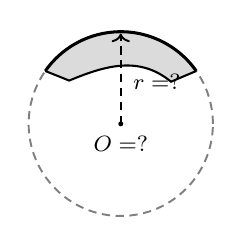
\begin{tikzpicture}[scale=0.45, every node/.style={font=\footnotesize, text=black}]
      \draw[black!50, line width=0.7pt, densely dashed] (0,0) circle (2.6);
      \fill[gray!28] (35:2.6) arc (35:145:2.6) -- (140:1.9) .. controls (105:1.7) and (75:2.0) .. (40:1.85) -- cycle;
      \draw[black, line width=1.1pt] (35:2.6) arc (35:145:2.6);
      \draw[black, line width=0.75pt] (145:2.6) -- (140:1.9) .. controls (105:1.7) and (75:2.0) .. (40:1.85) -- (35:2.6);
      \fill[black] (0,0) circle (2pt);
      \draw[black, line width=0.7pt, densely dashed, ->] (0,0) -- (90:2.55);
      \node[below=1pt] at (0,0) {$O = ?$};
      \node[right=1pt] at (0,1.2) {$r = ?$};
    \end{tikzpicture}
  \end{minipage}
\end{tcolorbox}

% ==================== ផ្នែកទី ២ ៖ E2 - EXPLORE ====================
\secbar{ផ្នែកទី ២ ៖ ពិសោធន៍ដែកឈានលើធាតុនៃរង្វង់ និងការកំណត់រង្វង់ (\enbf{E2 — Explore})}{\en{11} នាទី (ពិភាក្សាដៃគូ)}

\textbf{(ក) ធាតុនៃរង្វង់ $C(O,r)$ (ទំ.១៩៧)៖} ពិនិត្យរូបរង្វង់ផ្ចិត $O$ កាំ $r$ ខាងឆ្វេង រួចបំពេញចន្លោះ៖\\[2pt]
\begin{minipage}[c]{5.2cm}
  \centering
  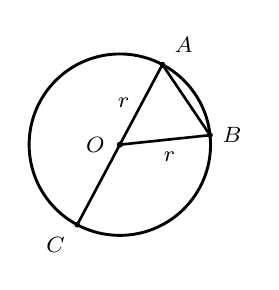
\begin{tikzpicture}[scale=0.48, every node/.style={font=\footnotesize, text=black}]
    \coordinate (O) at (0,0);
    \coordinate (A) at (62:2.4);
    \coordinate (C) at (242:2.4);
    \coordinate (B) at (6:2.4);
    \draw[black, line width=1.05pt] (O) circle (2.4);
    \draw[black, line width=0.95pt] (A)--(C) (A)--(B) (O)--(B);
    \fill[black] (O) circle (2.3pt) (A) circle (2.1pt) (B) circle (2.1pt) (C) circle (2.1pt);
    \node[left=2pt] at (O) {$O$};
    \node[above right=1pt] at (A) {$A$};
    \node[right=1pt] at (B) {$B$};
    \node[below left=1pt] at (C) {$C$};
    \node[left=1pt] at ($(O)!0.52!(A)$) {$r$};
    \node[below=1pt] at ($(O)!0.55!(B)$) {$r$};
  \end{tikzpicture}
\end{minipage}\hfill
\begin{minipage}[c]{13.3cm}
  \begin{enumerate}[label=\enbf{\arabic*.}, leftmargin=1.4em, itemsep=3pt, topsep=1pt]
    \item ប្រៀបធៀបប្រវែងពីផ្ចិត $O$ ទៅចំណុចលើរង្វង់៖ $OA =$ \blank{1.1cm} $=$ \blank{1.1cm} $= r$។
    \item អង្កត់ $AB$ ភ្ជាប់ពីរចំណុចលើរង្វង់ ហៅថា \textbf{អង្កត់\blank{2.0cm}}។
    \item អង្កត់ធ្នូ $AC$ ដែលគូសកាត់តាមផ្ចិត $O$ ហៅថា \textbf{អង្កត់\blank{2.0cm}} ហើយ $AC =$ \blank{0.9cm} $\times r$។
  \end{enumerate}
\end{minipage}

\vspace{3pt}
\textbf{(ខ) ពិសោធន៍សង់រង្វង់ដោយដែកឈានទាំង ៤ ករណី (ទំ.១៩៧--១៩៨)៖} ប្រើដែកឈានសាកល្បងសង់លើប្រអប់ទាំង ៤ ខាងក្រោម៖\\[2pt]
\renewcommand{\arraystretch}{1.18}
\begin{tabular}{|p{4.35cm}|p{4.45cm}|p{4.45cm}|p{4.45cm}|}
  \hline
  \cellcolor{headgray}\centering\textbf{១. តាម ១ ចំណុច $A$} &
  \cellcolor{headgray}\centering\textbf{២. តាម ២ ចំណុច $A, B$} &
  \cellcolor{headgray}\centering\textbf{៣. តាម ៣ ចំណុចមិនរត់ត្រង់គ្នា} &
  \cellcolor{headgray}\centering\arraybackslash\textbf{៤. អន្ទាក់ POE៖ រត់ត្រង់គ្នា} \\[2pt]
  \hline
  \centering
  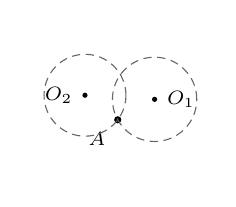
\begin{tikzpicture}[scale=0.52, every node/.style={font=\scriptsize, text=black}]
    \fill[black] (0,0) circle (2.5pt) node[below left=1pt] {$A$};
    \draw[black!60, densely dashed] (0.9,0.5) circle ({veclen(0.9,0.5)});
    \draw[black!60, densely dashed] (-0.8,0.6) circle ({veclen(0.8,0.6)});
    \fill[black] (0.9,0.5) circle (1.8pt) node[right=1pt] {$O_1$};
    \fill[black] (-0.8,0.6) circle (1.8pt) node[left=1pt] {$O_2$};
    \path (-2.2,-1.45) rectangle (2.2,2.25);
  \end{tikzpicture}
  \par ចំនួនរង្វង់៖ \blank{2.1cm}
  &
  \centering
  \begin{tikzpicture}[scale=0.52, every node/.style={font=\scriptsize, text=black}]
    \coordinate (A) at (-1.3,0); \coordinate (B) at (1.3,0);
    \draw[black, line width=0.8pt] (A)--(B);
    \draw[black, line width=0.85pt, densely dashed] (0,-1.35)--(0,2.1);
    \rightbox[0.18cm]{B}{0,0}{0,1.2}
    \tickone{A}{0,0}\tickone{0,0}{B}
    \fill[black] (A) circle (2.4pt) node[below=1pt] {$A$} (B) circle (2.4pt) node[below=1pt] {$B$};
    \fill[black] (0,1.05) circle (2pt) node[right=1pt] {$O_1$};
    \node[left=1pt] at (0,1.85) {$d$};
    \path (-2.2,-1.45) rectangle (2.2,2.25);
  \end{tikzpicture}
  \par ផ្ចិតស្ថិតលើ៖ \blank{2.1cm}
  &
  \centering
  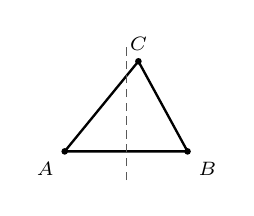
\begin{tikzpicture}[scale=0.52, every node/.style={font=\scriptsize, text=black}]
    \coordinate (A) at (-1.5,-0.55); \coordinate (B) at (1.5,-0.55); \coordinate (C) at (0.3,1.65);
    \draw[black, line width=0.85pt] (A)--(B)--(C)--cycle;
    \draw[black!65, densely dashed] (0,-1.25)--(0,2.0);
    \fill[black] (A) circle (2.3pt) node[below left=0.5pt] {$A$} (B) circle (2.3pt) node[below right=0.5pt] {$B$} (C) circle (2.3pt) node[above=0.5pt] {$C$};
    \path (-2.2,-1.45) rectangle (2.2,2.25);
  \end{tikzpicture}
  \par ចំនួនរង្វង់៖ \blank{2.1cm}
  &
  \centering\arraybackslash
  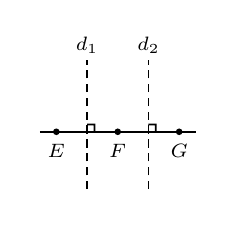
\begin{tikzpicture}[scale=0.52, every node/.style={font=\scriptsize, text=black}]
    \draw[black, line width=0.85pt] (-1.9,0.2)--(1.9,0.2);
    \draw[black, densely dashed] (-0.75,-1.2)--(-0.75,1.95) node[above=-1pt] {$d_1$};
    \draw[black, densely dashed] (0.75,-1.2)--(0.75,1.95) node[above=-1pt] {$d_2$};
    \rightbox[0.18cm]{0,0.2}{-0.75,0.2}{-0.75,1.2}
    \rightbox[0.18cm]{1.5,0.2}{0.75,0.2}{0.75,1.2}
    \fill[black] (-1.5,0.2) circle (2.3pt) node[below=1pt] {$E$} (0,0.2) circle (2.3pt) node[below=1pt] {$F$} (1.5,0.2) circle (2.3pt) node[below=1pt] {$G$};
    \path (-2.2,-1.45) rectangle (2.2,2.25);
  \end{tikzpicture}
  \par $d_1 \parallel d_2 \Rightarrow$ \blank{1.7cm} រង្វង់ \\[3pt]
  \hline
\end{tabular}

% ==================== ផ្នែកទី ៣ ៖ E3 - EXPLAIN ====================
\secbar{ផ្នែកទី ៣ ៖ សំយោគនិយមន័យ ទ្រឹស្ដីបទ និងធនាគារហេតុផល (\enbf{E3 — Explain})}{\en{6} នាទី}

\begin{tcolorbox}[
  enhanced, sharp corners, colback=white, colframe=black,
  boxrule=1.0pt, boxsep=2pt, top=3.5pt, bottom=3.5pt, left=6pt, right=6pt, after skip=3.5pt
]
  $\bullet$ \textbf{និយមន័យ៖} សំណុំចំណុចក្នុងប្លង់ដែលមានចម្ងាយស្មើនឹង \blank{1.0cm} ពីផ្ចិត $O$ ហៅថា \textbf{រង្វង់} កំណត់ដោយ \blank{1.8cm}។\\[2.5pt]
  $\bullet$ \textbf{ទ្រឹស្ដីបទ (ទំ.១៩៨)៖} តាមបីចំណុចដែល \textbf{\blank{4.2cm}} គេអាចគូសបានរង្វង់ \textbf{\blank{2.4cm}} ដែលកាត់តាមចំណុចទាំងបីនោះ (ផ្ចិត $O$ គឺជាចំណុចប្រសព្វនៃ \textbf{\blank{3.0cm}} របស់ជ្រុងត្រីកោណ $ABC$)។\\[3pt]
  {\fontsize{9pt}{12.5pt}\selectfont\renewcommand{\arraystretch}{1.18}
  \begin{tabular}{|p{4.1cm}|p{3.9cm}|p{9.2cm}|}
    \hline
    \cellcolor{headgray}\centering\textbf{ចំណុចដែលគេឱ្យ} &
    \cellcolor{headgray}\centering\textbf{ចំនួនរង្វង់គូសបាន} &
    \cellcolor{headgray}\centering\arraybackslash\textbf{ទីតាំងនៃផ្ចិតរង្វង់} \\[2pt]
    \hline
    ១ ចំណុច ($A$) & ច្រើនរាប់មិនអស់ & គ្រប់ចំណុចក្នុងប្លង់ (លើកលែង $A$ បើ $r>0$) \\[1.5pt]
    \hline
    ២ ចំណុច ($A, B$) & ច្រើនរាប់មិនអស់ & ស្ថិតនៅលើ \textbf{មេដ្យាទ័រ} នៃអង្កត់ $AB$ \\[1.5pt]
    \hline
    ៣ ចំណុចមិនរត់ត្រង់គ្នា & \textbf{តែ ១ គត់} & ប្រសព្វមេដ្យាទ័រទាំងបីនៃជ្រុង $\tri{ABC}$ \\[1.5pt]
    \hline
    ៣ ចំណុចរត់ត្រង់គ្នា & \textbf{$0$ រង្វង់ (គូសមិនបាន)} & គ្មាន (ព្រោះមេដ្យាទ័រទាំងពីរស្របគ្នា $d_1 \parallel d_2$) \\[1.5pt]
    \hline
  \end{tabular}}\\[3pt]
  \textbf{ធនាគារហេតុផល៖} \cnum{1} និយមន័យរង្វង់ $C(O,r)$ $\;\vert\;$ \cnum{2} លក្ខណៈមេដ្យាទ័រ ($M \in d \Leftrightarrow MA=MB$) $\;\vert\;$ \cnum{3} លក្ខណៈឆ្លងនៃសមភាព។
\end{tcolorbox}

% ប្រអប់ផ្ទៀងផ្ទាត់ការយល់ច្រឡំភ្លាមៗ ដើម្បីប្រើក្រដាសទំព័រទី១ ឱ្យអស់លទ្ធភាព
\begin{tcolorbox}[
  enhanced, sharp corners, colback=panelgray, colframe=black,
  boxrule=0.85pt, left=6pt, right=6pt, top=3pt, bottom=3pt
]
  \textbf{ផ្ទៀងផ្ទាត់ការយល់ដឹងភ្លាមៗ (គូសធីក \chkbox\ ពិត ឬ មិនពិត ដើម្បីបំបែកការយល់ច្រឡំ)៖}\\[2pt]
  ១. អង្កត់ផ្ចិតនៃរង្វង់ $C(O,r)$ មានប្រវែងស្មើនឹងពីរដងនៃកាំ ($d = 2r$)។ \hfill \chkbox\ ពិត \hspace{0.35cm} \chkbox\ មិនពិត\\[2pt]
  ២. តាមបីចំណុចណាក៏ដោយក្នុងប្លង់ គេតែងតែអាចគូសរង្វង់កាត់តាមបាន ១ ជានិច្ច។ \hfill \chkbox\ ពិត \hspace{0.35cm} \chkbox\ មិនពិត\\[2pt]
  ៣. ចំណុចផ្ចិត $O$ គឺជាចំណុចមួយដែលស្ថិតនៅលើខ្សែរង្វង់ $C(O,r)$ ($r > 0$)។ \hfill \chkbox\ ពិត \hspace{0.35cm} \chkbox\ មិនពិត
\end{tcolorbox}

\newpage

% ==================== ទំព័រទី ២ ៖ E4, E5 និងកិច្ចការផ្ទះ ====================
\secbar{ផ្នែកទី ៤ ៖ សម្រាយបញ្ជាក់លំហាត់គំរូ និងទីតាំងចំណុចធៀបនឹងរង្វង់ (\enbf{E4 — Elaborate})}{\en{10} នាទី (ទំ.១៩៨)}

\begin{tcolorbox}[
  enhanced, sharp corners, colback=white, colframe=black,
  boxrule=0.95pt, boxsep=2pt, top=4pt, bottom=4pt, left=6pt, right=6pt, after skip=4.5pt
]
  \begin{minipage}[c]{12.2cm}
    \textbf{១. លំហាត់គំរូ (ទំ.១៩៨)៖} គេមានបីចំណុច $A, B$ និង $C$ មិនស្ថិតនៅលើបន្ទាត់តែមួយ។ ចូរបំពេញសម្រាយបញ្ជាក់ថាចំណុច $A, B, C$ ស្ថិតនៅលើរង្វង់តែមួយគត់៖
    \begin{itemize}[leftmargin=1.2em, itemsep=2.5pt, topsep=2pt]
      \item សង់មេដ្យាទ័រ $MN$ នៃអង្កត់ $AC$ និងមេដ្យាទ័រ $PQ$ នៃអង្កត់ $AB$។
      \item ដោយ $A, B, C$ មិនរត់ត្រង់គ្នា នោះ $MN$ និង $PQ$ ប្រសព្វគ្នាត្រង់ចំណុច \blank{1.0cm} តែមួយគត់។
      \item ដោយ $O \in MN$ (មេដ្យាទ័រនៃ $AC$) គេបាន $OA =$ \blank{1.2cm} (តាមហេតុផលលេខ \blank{0.8cm})។
      \item ដោយ $O \in PQ$ (មេដ្យាទ័រនៃ $AB$) គេបាន $OA =$ \blank{1.2cm} (តាមហេតុផលលេខ \blank{0.8cm})។
      \item តាម \cnum{3} គេទាញបាន $OA =$ \blank{1.1cm} $=$ \blank{1.1cm} $= r$។ ដូចនេះ រង្វង់ $C(O, OA)$ កាត់តាម $A, B, C$ តែមួយគត់ (តាម \cnum{1})។
    \end{itemize}
  \end{minipage}\hfill
  \begin{minipage}[c]{5.8cm}
    \centering
    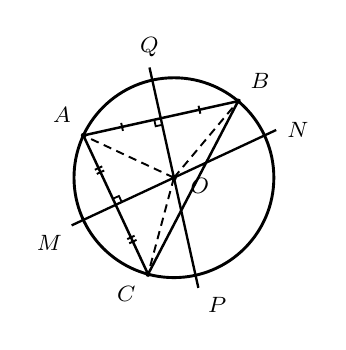
\begin{tikzpicture}[scale=0.47, every node/.style={font=\footnotesize, text=black}]
      \coordinate (O) at (0,0);
      \def\R{2.7}
      \coordinate (A) at (155:\R);
      \coordinate (B) at (50:\R);
      \coordinate (C) at (-105:\R);
      \coordinate (M1) at ($(A)!0.5!(C)$);
      \coordinate (M2) at ($(A)!0.5!(B)$);
      \coordinate (Mend) at (205:3.05);
      \coordinate (Nend) at (25:3.05);
      \coordinate (Qend) at (102.5:3.05);
      \coordinate (Pend) at (-77.5:3.05);
      \draw[black, line width=1.05pt] (O) circle (\R);
      \draw[black, line width=0.9pt] (A)--(B)--(C)--cycle;
      \draw[black, line width=0.7pt, densely dashed] (O)--(A) (O)--(B) (O)--(C);
      \draw[black, line width=0.85pt] (Mend) -- (Nend);
      \draw[black, line width=0.85pt] (Qend) -- (Pend);
      \rightbox[0.18cm]{A}{M1}{O}\rightbox[0.18cm]{A}{M2}{O}
      \ticktwo{A}{M1}\ticktwo{M1}{C}\tickone{A}{M2}\tickone{M2}{B}
      \fill[black] (O) circle (2.3pt) (A) circle (2pt) (B) circle (2pt) (C) circle (2pt);
      \node[above left=1pt] at (A) {$A$}; \node[above right=1pt] at (B) {$B$}; \node[below left=1pt] at (C) {$C$};
      \node[right=2.5pt] at (0,-0.22) {$O$};
      \node[below left=0pt] at (Mend) {$M$}; \node[right=0.5pt] at (Nend) {$N$};
      \node[above=0.5pt] at (Qend) {$Q$}; \node[below right=0pt] at (Pend) {$P$};
    \end{tikzpicture}
  \end{minipage}
\end{tcolorbox}

\begin{tcolorbox}[
  enhanced, sharp corners, colback=panelgray, colframe=black,
  boxrule=0.85pt, left=6pt, right=6pt, top=3pt, bottom=3pt, after skip=4.5pt
]
  \textbf{២. អនុវត្តរហ័ស៖} គេមានរង្វង់ $C(O, 3.5\unit{cm})$។ ប្រវែងអង្កត់ផ្ចិតគឺ $d = 2r =$ \blank{1.3cm} $\unit{cm}$។ ចូរបំពេញពាក្យ \textbf{«ក្នុងរង្វង់»}, \textbf{«លើរង្វង់»} ឬ \textbf{«ក្រៅរង្វង់»}៖\\[2pt]
  (ក) បើ $OM = 2.8\unit{cm} \Rightarrow M$ ស្ថិតនៅ \blank{2.2cm} $\;\vert\;$
  (ខ) បើ $ON = 3.5\unit{cm} \Rightarrow N$ ស្ថិតនៅ \blank{2.2cm} $\;\vert\;$
  (គ) បើ $OP = 4.2\unit{cm} \Rightarrow P$ ស្ថិតនៅ \blank{2.2cm}។
\end{tcolorbox}

% ==================== ផ្នែកទី ៥ ៖ E5 - EVALUATE ====================
\secbar{ផ្នែកទី ៥ ៖ ប្រតិបត្តិសង់រង្វង់ដោយដែកឈាន និងបិទបេសកកម្ម (\enbf{E5 — Evaluate})}{\en{10} នាទី (ទំ.១៩៨)}

\begin{tcolorbox}[
  enhanced, sharp corners, colback=white, colframe=black,
  boxrule=0.95pt, boxsep=2pt, top=4pt, bottom=4pt, left=6pt, right=6pt, after skip=4.5pt
]
  \textbf{១. ប្រតិបត្តិ (ទំ.១៩៨)៖} អង្កត់ $AB$ ខាងក្រោមមានប្រវែងពិត $AB = 6\unit{cm}$ (មាត្រដ្ឋាន $1:1$)។ ចូរប្រើដែកឈានគូសគូរង្វង់ ឬគណនាប្រៀបធៀបផលបូកកាំ $r_1 + r_2$ នឹង $AB = 6\unit{cm}$ រួចកត់ត្រាចំនួនចំណុចប្រសព្វ៖
  \begin{center}
    \vspace{-2pt}
    \begin{tikzpicture}[x=1cm, y=1cm, every node/.style={font=\footnotesize, text=black}]
      % បន្ទប់សង់ពិត 1:1 ប្រវែង AB = 6 cm ជាមួយក្រិត 1 cm
      \draw[gray!40, line width=0.4pt] (-1.8,-1.25) rectangle (7.8,1.25);
      \draw[black, line width=1.15pt] (0,0)--(6,0);
      \foreach \x in {0,1,2,3,4,5,6} {
        \draw[black, line width=0.7pt] (\x,-0.10)--(\x,0.10);
      }
      \fill[black] (0,0) circle (2.2pt) node[below=3pt] {$A\;(0\unit{cm})$};
      \fill[black] (6,0) circle (2.2pt) node[below=3pt] {$B\;(6\unit{cm})$};
      \node[above=2pt] at (3,0.08) {$AB = 6\unit{cm}$ (ក្រិត $1\unit{cm}$ ពិត)};
    \end{tikzpicture}
    \vspace{-3pt}
  \end{center}
  \renewcommand{\arraystretch}{1.22}
  \begin{tabular}{|p{5.8cm}|p{5.8cm}|p{5.8cm}|}
    \hline
    \cellcolor{headgray}\centering\textbf{ក. $C(A, 2\unit{cm})$ និង $C(B, 4\unit{cm})$} &
    \cellcolor{headgray}\centering\textbf{ខ. $C(A, 3\unit{cm})$ និង $C(B, 5\unit{cm})$} &
    \cellcolor{headgray}\centering\arraybackslash\textbf{គ. $C(A, 1\unit{cm})$ និង $C(B, 2\unit{cm})$} \\[2pt]
    \hline
    $r_1 + r_2 = 2 + 4 =$ \blank{0.9cm} $\unit{cm}$ ($= AB$)\par
    ចំនួនចំណុចប្រសព្វ៖ \blank{1.2cm} ចំណុច &
    $r_1 + r_2 = 3 + 5 =$ \blank{0.9cm} $\unit{cm}$ ($> AB$)\par
    ចំនួនចំណុចប្រសព្វ៖ \blank{1.2cm} ចំណុច &
    \arraybackslash $r_1 + r_2 = 1 + 2 =$ \blank{0.9cm} $\unit{cm}$ ($< AB$)\par
    ចំនួនចំណុចប្រសព្វ៖ \blank{1.2cm} ចំណុច \\[3pt]
    \hline
  \end{tabular}
\end{tcolorbox}

\begin{tcolorbox}[
  enhanced, sharp corners, colback=white, colframe=black,
  boxrule=0.95pt, boxsep=2pt, top=3.5pt, bottom=3.5pt, left=6pt, right=6pt, after skip=4.5pt
]
  \textbf{២. បិទបេសកកម្ម E1 (បំណែកចានបុរាណ)៖} គេត្រូវដៅយ៉ាងតិច \blank{1.0cm} ចំណុចមិនរត់ត្រង់គ្នា $A, B, C$ លើគែមចាន រួចសង់ \textbf{\blank{2.8cm}} នៃអង្កត់ធ្នូ $AB$ និង $BC$ ឱ្យប្រសព្វគ្នាត្រង់ផ្ចិតដើម $O$ តែមួយគត់!\\[3pt]
  \textbf{៣. Exit Check (៦០ វិនាទី)៖} បើបីចំណុច $E, F, G$ ស្ថិតនៅលើបន្ទាត់ត្រង់តែមួយ តើគេអាចគូសរង្វង់កាត់តាមចំណុចទាំងបីបានប៉ុន្មាន?\\
  \chkbox\ \textbf{A.} $0$ រង្វង់ (គូសមិនបាន) \hspace{0.5cm}
  \chkbox\ \textbf{B.} $1$ រង្វង់គត់ \hspace{0.5cm}
  \chkbox\ \textbf{C.} $2$ រង្វង់ \hspace{0.5cm}
  \chkbox\ \textbf{D.} ច្រើនរាប់មិនអស់
\end{tcolorbox}

% ==================== កិច្ចការផ្ទះ (ជំហានទី ៥) ====================
\begin{tcolorbox}[
  enhanced, sharp corners, colback=panelgray, colframe=black,
  boxrule=1.0pt, boxsep=2pt, top=3.5pt, bottom=3.5pt, left=6pt, right=6pt
]
  {\muol\fontsize{9.0pt}{13pt}\selectfont កិច្ចការផ្ទះ (សៀវភៅសិក្សាគោល ទំព័រ ២០៤ — ត្រៀមរ៉ាប់ព័រទ័រវាស់មុំសម្រាប់ម៉ោងក្រោយ)}\\[2pt]
  $\bullet$ \textbf{លំហាត់ទី ៦ (ទំ.២០៤)៖} ត្រីកោណសម័ង្ស $ABC$ មាន $I, J, K$ ជាចំណុចកណ្ដាលរៀងគ្នានៃ $AB, BC, CA$។ ស្រាយបញ្ជាក់ថា $B, I, K, C$ ស្ថិតនៅលើរង្វង់តែមួយដែលមានផ្ចិត $J$ (ណែនាំ៖ បង្ហាញថា $JB = JI = JK = JC = \frac{1}{2}AB$ តាមលក្ខណៈអង្កត់មធ្យមត្រីកោណ)។\\
  $\bullet$ \textbf{លំហាត់ទី ៧ (ទំ.២០៤)៖} ចតុកោណ $ABCD$ មានអង្កត់ទ្រូងទាំងពីរកែងគ្នា ($AC \perp BD$) ហើយ $M, N, R, S$ ជាចំណុចកណ្ដាលជ្រុងទាំងបួន។ ស្រាយបំភ្លឺថា $M, N, R, S$ ស្ថិតនៅលើរង្វង់តែមួយ (ណែនាំ៖ បង្ហាញថា $MNRS$ ជាចតុកោណកែង)។
\end{tcolorbox}

\end{document}
